\documentclass[a4paper, 12pt, final]{hitec}
\usepackage[T1]{fontenc} % this makes text underscore look better
\usepackage{textcomp} % load symbol definitions
\usepackage{underscore} % allows the use of _ in text without escaping
\usepackage[english]{babel}
\usepackage[english]{isodate}
\usepackage[parfill]{parskip}
\usepackage{ragged2e}
\usepackage{appendix}
%\usepackage[none]{hyphenat}% enable to switch off hypenation
\usepackage{times}
\usepackage{setspace}
\usepackage{enumitem}% http://ctan.org/pkg/enumitem
\usepackage{tabulary}
\usepackage{longtable}
\usepackage{inputenc}
\usepackage{amssymb}
\usepackage{amsfonts}
\usepackage[pdftex]{graphicx}
\usepackage[dvipsnames]{xcolor}
\usepackage{subcaption}
\usepackage{wrapfig}
\usepackage{float}
\usepackage{fancyvrb}
\usepackage{alltt}
\usepackage{moreverb}
\usepackage[singlelinecheck=false, justification=centering]{caption}
\usepackage{booktabs,array}
\newcolumntype{?}{!{\vrule width 1pt}}
\makeatletter
\def\thickhline{%
  \noalign{\ifnum0=`}\fi\hrule \@height \thickarrayrulewidth \futurelet
   \reserved@a\@xthickhline}
\def\@xthickhline{\ifx\reserved@a\thickhline
               \vskip\doublerulesep
               \vskip-\thickarrayrulewidth
             \fi
      \ifnum0=`{\fi}}
\makeatother

\newlength{\thickarrayrulewidth}
\setlength{\thickarrayrulewidth}{2\arrayrulewidth}
% for more info on hyperref package see http://en.wikibooks.org/wiki/LaTeX/Packages/Hyperref
\usepackage[pdftex,colorlinks=true,linkcolor=BlueViolet]{hyperref}

\addto{\captionsenglish}{\renewcommand{\abstractname}{Executive Summary}}

\usepackage{lastpage}

\renewcommand{\baselinestretch}{1.1}

%% important to have floats such as tables stick to the top if option [t!] is used
\makeatletter
\setlength{\@fptop}{0pt}
\makeatother

\let\footruleskip\undefined
\usepackage{fancyhdr}

\addto\captionsenglish{% Replace "english" with the language you use
  \renewcommand{\contentsname}%
    {Table of Contents}%
}

\title{Berlin Airport Asset Acquisition Application User Manual}
\author{Your Company}
\date{\today}
\usepackage{hyperxmp}
\hypersetup{
    pdftitle={User Manual: how to use you system},
    pdfauthor={Your Company},
    pdfsubject={Once sentence description on the manual.},
    pdfcopyright={Copyright (C) 2019 by Your Company.  All rights reserved.}
}

\makeatletter
\let\thetitle\@title
\let\theauthor\@author
\let\thedate\@date
\makeatother

\pagestyle{fancy}
\fancyhf{}
%\rhead{\theauthor}
\lhead{\thetitle}
\cfoot{\thepage}

\captionsetup[table]{font=footnotesize, labelfont=bf}
\captionsetup[figure]{font=footnotesize, labelfont=bf}
\captionsetup[subfigure]{font=scriptsize, labelfont=bf}

%----------------------------------------------------------------------------------------
%	DOCUMENT MARGINS
%----------------------------------------------------------------------------------------

%\textwidth 6.75in
\textheight 25cm
%\oddsidemargin -.25in
%\evensidemargin -.25in
\topmargin -1cm
%\longindentation 0.50\textwidth
%\parindent 0.2in

%----------------------------------------------------------------------------------------
%	TIKZ magic
%----------------------------------------------------------------------------------------

\usepackage{tikz}
\usetikzlibrary{shadows}

\newcommand*\keystroke[1]{%
  \tikz[baseline=(key.base)]
    \node[%
      draw,
      fill=white,
      drop shadow={shadow xshift=0.25ex,shadow yshift=-0.25ex,fill=black,opacity=0.75},
      rectangle,
      rounded corners=2pt,
      inner sep=1pt,
      line width=0.5pt,
      font=\scriptsize\sffamily,
      minimum width=1.2em
    ](key) {#1\strut};
}

%----------------------------------------------------------------------------------------
%	DOCUMENT CONTENT
%----------------------------------------------------------------------------------------

\begin{document}
	\onehalfspacing
	\pagenumbering{roman}
  \begin{titlepage}
      \centering
        \vspace*{0.5 cm}
      \rule{\linewidth}{0.2 mm} \\[0.4cm]
      \begin{spacing}{1.1}
        \huge \bfseries Berlin Airport Asset Acquisition Application\\[0.3cm]
        \LARGE User Manual
      \end{spacing}
      \rule{\linewidth}{0.2 mm} \\[1 cm]
      \large \bfseries Team Berlin: \\
        Myroslava Romaniuk : code + user manual \\
        Andrian Hevalo : user manual \\
        Yaroslav Boiko : code \\
        Daryna Dzhala : code \\
        Oleksandr Potapov : code
      \clearpage
      
      \setcounter{page}{1}
      \justifying Synopsis about the system:

      The file you are reading was written to make this project easy to use,
      and the idea behind it understanable. It is a quick guide into project
      features, user stories, as well as how to start using it.
      
      In general, the project is a Java application asset management platform
      created for the Berlin airport.

      Basically, the main basis for the platform was already implemented,
      but our main task was to extend its functionality by implementing user stories
      and therefore satisfying the needs of our various users. 
      \clearpage
        
      \setcounter{tocdepth}{3}
      \tableofcontents
      \clearpage
  \end{titlepage}

  \pagenumbering{arabic}
  \section{TG background}\label{sec:01}
  TG exists to remove many low level technical obstacles that are
  often associated with building sophisticated transnational applications
  such as Enterprise Asset Maintenance (EAM) or Enterprise Resource Planning
  (ERP) systems. We have successfully used TG for developing large-scale and
  mission-critical enterprise applications.

  With TG, we look at the system design as the decomposition problem,
  which can be solved successfully with the right approach in the right context.
  TG establishes a well defined pattern for modelling business domains,
  including domain entities, processes and their inter-dependencies (down to the
  level of properties with automatic revalidation support).
  
  At the code level the
  description of the domain model is achieved by using a small set of base classes
  and various annotations. Together these constitute what we refer to as "Entity
  Definition Language" (EDL), which is complemented by "Entity Query Language"
  (EQL) for data querying (relational databases).

  The setup of TG essentially served as the foundation for our system.
  Setting the maven dependency, we got the initial building blocks needed
  to continue with expanding the functionality and eventually building our own
  system which implements the requirements from user stories. As mentioned above,
  the TG setup consisted of TG-specific classes and annotations that provide the
  tools and guide the model-driven development of the platform.
  \clearpage

  \section{Main ideas for our version of the platform}\label{sec:02}
  \hyperref[sec:01_01:fig:01]{Fig.~\ref*{sec:01_01:fig:01}} illustrates the main menu of your system.
	\begin{figure}[!htbp]
	\centering
	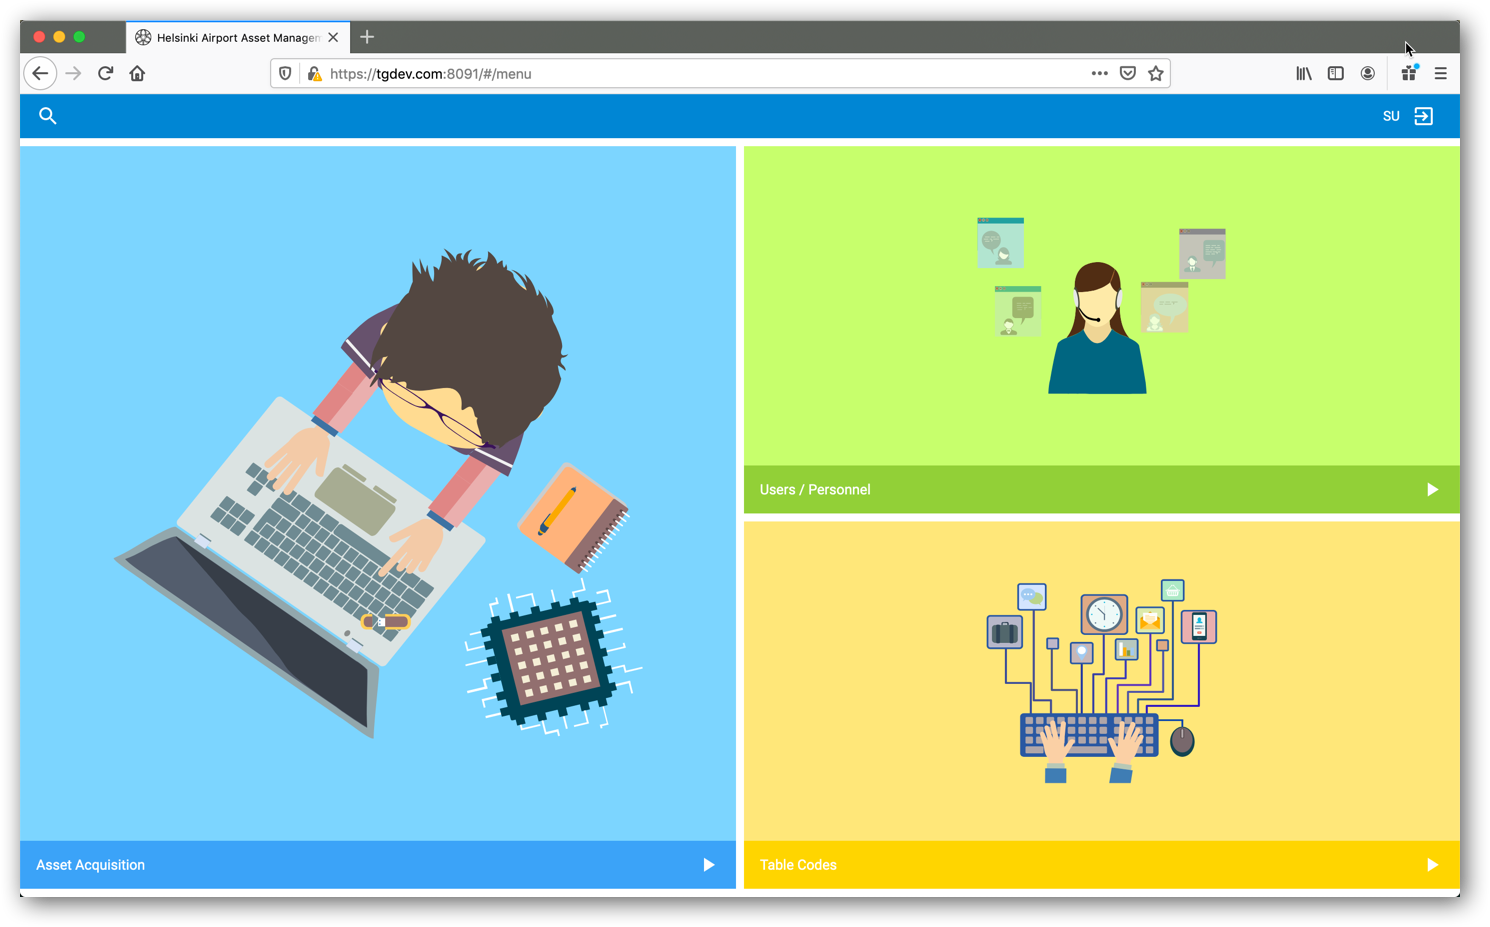
\includegraphics[width=0.95\linewidth]{images/01-main-menu.png}
	\caption{Application main menu.}\label{sec:01_01:fig:01}
  \end{figure}
  \clearpage

  \section{User stories}\label{sec:03}
  Ihe idea behind the user stories is to provide the project we are working on with clarity. 
  Also the purpose of user stories in airport project is to implement the functionality needed
  for convinient project use (system engineer, Maintenance Planner, Maintenance Scheduler, Accounant).
  It was stated that 6th and yth user stories aren't needed for implementation, therefore we implemented all expaect 6 and 7.
  It would be great specify the purpose of each issue but i will try to sum the up:
  AC1: defining an Asset class 
  AC2: add types for Asset class
  AC3: add Service status
  AC4: add Condition ratings
  The rest are directly related to AC1 - AC4.
  For some issues we implemented tests that check the correctness of the implementation.
  todo: describe the idea for user stories (satisfying needs of users
  who comprise of airport workers), the functionality that needed to be
  implemented and descriptions and requirements of each particular issue.
  and again, explictly state which of the issues were implemented.
  \clearpage

  \section{Tiles: Asset Acquisition}\label{sec:04}
  Asset Acquisition part is for adding new functionality to the project and 
  prepare it for user use.
  Asset Owner: Approves Asset Management Plans and Asset renewal forecasts.
  Maintenance Planner: Responsible for ensuring the Maintenance Register is up-to-date and accurate.
  Maintenance Scheduler: Responsible for scheduling Asset Management delivery services.
  System Engineer: Support and admin for CMMS and related tools.
  Accountant: Represents the Finance team.
  todo: describe the model and parts of the system that belong
  to the asset acquision module + provide instruction for what
  actions can be done in the application (UI side).
  \clearpage

  \section{Tiles: Users / Personnel}\label{sec:05}
  .
  .
  .
  todo: describe the model and parts of the system that belong
  to the users / personnel module + provide instruction for what
  actions can be done in the application (UI side).
  \clearpage

  \section{Tiles: Table Codes}\label{sec:06}
  .
  .
  .
  todo: describe the model and parts of the system that belong
  to the table codes module + provide instruction for what
  actions can be done in the application (UI side). also mention
  the connections some of the table codes entities have to the
  entities on the asset acquision side.
  \clearpage

  \section{Project Summary}\label{sec:07}
  The main purpose of the project is to learn to implement and work with 
  java application with UI and databases. We definately had a lot of
  problems while working on a project due to not decent knowledge and experience.
  Fortunatelly, we maintained the goal! 
  
  All parts of the project are working together (UI, server, back-end).

  The functionality we added to the project is working well and is partially covered by tests.
  Tests helped us to better understand the issues and avoid bugs.

  The project was in development during the semester but most job was done in last month
  due to upcoming deadline. We managed to complete almost everything that was needed. 
  For instance: tests, implementation of user stories and user guide. 
  todo:
  include a summary in which you talk about
  \begin{enumerate}
    \item the goal of the project and whether it was reached
    \item summarise the parts of the program and how they work together
    \item add that all functionality is working and covered by tests
    \item mention the dates the project was in development and which tasks have been completed
  \end{enumerate}
  \clearpage
\end{document}